\mysection{Experimental Results}

Before showing the results of the simulations, it is interesting to discuss the experimental results for the studied observables. They indicate that jets suffer modifications due to interactions with the dense and hot medium created in relativistic heavy-ion collisions. The first of these, and most inclusive one is the jet $p_T$. We can observe in Figure \ref{exp_jet_pt} that the PbPb spectrum is is suppressed when compared to the pp spectrum. The same trend is observed when central and semi-peripheral collisions are compared: the former is more suppressed than the later. This indicates that there is suppression of jets for PbPb collisions, and that this suppression is also related to centrality. The fact that it varies with the centrality is also an evidence that this suppression has its origin in the interaction with the medium. In the Figure \ref{exp_jet_pt_raa} we see that the PbPb spectrum can be $20\%$ that of pp for lower transverse momentum, and saturates at no more than $60\%$ for higher values of $p_T$.

\begin{figure}
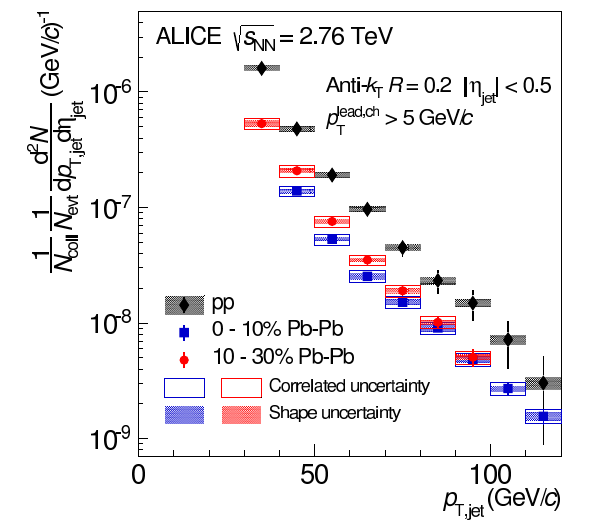
\includegraphics[width=0.6\textwidth]{images/exp_jet_pt.png}
\caption[Experimental Jet $p_T$]{The spectra of $R = 0.2$ jets with a leading track requirement of $5 \, {\rm GeV/c}$ in $0-10\%$ and $10-30\%$ most central Pb–Pb collisions scaled by $1/N_{coll}$ and in inelastic pp collisions at $\sqrt{s_{NN}} = 2.76 \, {\rm TeV}$. Plot from \cite{alice_collaboration_measurement_2015}}
\label{exp_jet_pt}
\end{figure}

\begin{figure}
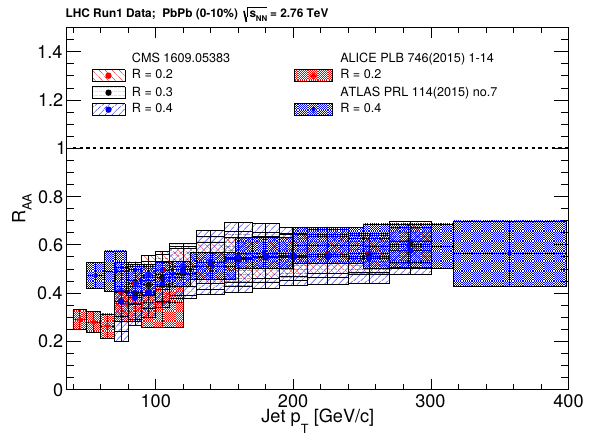
\includegraphics[width=0.6\textwidth]{images/exp_jet_pt_raa.png}
\caption[Experimental Jet $p_T$ $R_{AA}$]{Jet $p_T$ $R_{AA}$ measured in different collaborations. Figure from \cite{connors_review_2017}.}
\label{exp_jet_pt_raa}
\end{figure}

There is also evidences that this suppression is path length dependent. This can be seen in Figure \ref{exp_jet_v2} where several measurements of $v_2$ are presented. The data in orange and in white circles are measurements of the $v_2$. They come from ALICE and CMS collaborations respectively. The fact that it grows linearly for lower $p_t$ is predicted by modeling collective behavior. For $p_T \gtrsim 5\,{\rm GeV}$, the particles are not usually thermalized. The description of the particles as Jet Quenching then comes into play. We see in the plot that the $v_2$ continues to be non-zero well above $5\,{\rm GeV}$. This indicates that the energy loss of this partons must be path length dependent. The fact that it depends also on centrality is evidence that this comes from the interaction of high energy partons with the medium. The data in black circles comes and in blue squares come from ALICE and ATLAS collaborations, respectively. This data is different from the previous cases since it uses reconstructed jets. ALICE reconstructs jets with the TPC, so only charged particles are included in the analysis. ATLAS uses the hadronic calorimeters, which means it measures full jets. This difference introduces a different scale for the measurements, since ALICE will not include neutral particles when clustering the jets. For semi-central and central collisions, the collaborations do not agree upon a re-scaling of jet momenta. ALICE measures a higher value for $v_2$.

\begin{figure}
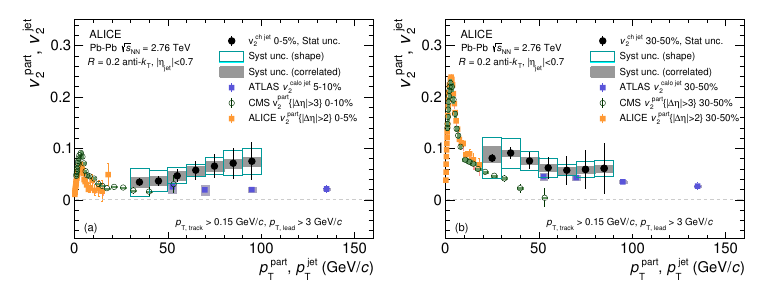
\includegraphics[width=1.0\textwidth]{images/exp_v2.png}
\caption[Experimental Jet $v_2$]{Jet $v_2$ measured in different collaborations. Figure from \cite{connors_review_2017}.}
\label{exp_jet_v2}
\end{figure}

In Figure \ref{exp_girth_ptd} we see measurements of the girth and $p_t^{D}$ for charged jets with small radius $(R=0.2)$ jets. The simulations for pp describe well the data for these observables\cite{alice_collaboration_medium_2018}. There is a modification if compared with the simulation also displayed in the plot. The girth indicates more collimated jets. The $p_t^D$ indicates harder fragmentation if compared to the pp case.

\begin{figure}
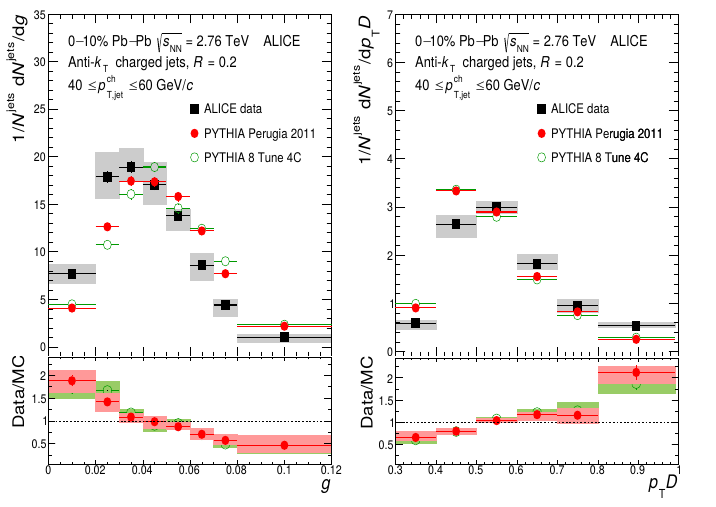
\includegraphics[width=1.0\textwidth]{images/exp_girth_ptd.png}
\caption[Experimental Girth and $p_t^{D}$]{Girth and $p_t^D$ measured by ALICE collaboration. Figure from \cite{alice_collaboration_medium_2018}.}
\label{exp_girth_ptd}
\end{figure}


Regarding jet mass, the first measurements can be seen in the Figure \ref{exp_jet_mass}. In the Figure, the mass measured in PbPb collisions is compared to pPb collisions. pp data for jet mass is well described by simulations. In \cite{alice_collaboration_first_2018} the comparison of pPb with simulations for pp show that there are no cold matter nuclear effects on this observable. So the comparison of PbPb with pPb would show only the effects of the hot QGP on the partons. For jets on the range $60-100 \, {\rm GeV}$ range, the jets in PbPb tend to have slightly lower mass than those of pPb. This indicates a broadening of the jet.

\begin{figure}
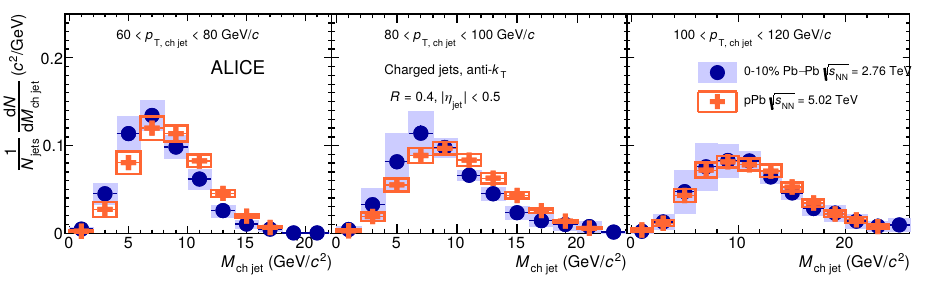
\includegraphics[width=1.0\textwidth]{images/exp_jet_mass.png}
\caption[Experimental Jet Mass]{Jet mass measured by ALICE collaboration. Figure from \cite{alice_collaboration_first_2018}.}
\label{exp_jet_mass}
\end{figure}

\mysection{JEWEL results}

JEWEL was developed to describe data from heavy-ion collisions. And it can reproduce most inclusive data. An example is displayed in Figure \ref{hadron_supression}. In the Figure we can see the prediction for neutral pion $p_t$ spectrum supression, as measured by PHENIX collaboration. It was one of the first results to indicate the phenomenum of Jet Quenching. In Figure \ref{charged_hadron_supression} we can see the supression for charged hadrons compared to data from ALICE and CMS collaborations. JEWEL describes this inclusive data really well. Also, in Figure \ref{jewel_jetpt_supression} we can see that the supression for reconstructed jets is also well described by JEWEL. The two Figures combined show that JEWEL can handle a wide energy range and different hadrochemistry well.

\begin{figure}
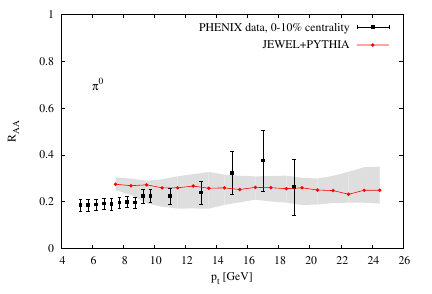
\includegraphics[width=0.8\textwidth]{images/hadron_supression.png}
\caption[Hadron $R_{AA}$]{Hadron $R_{AA}$ as measured by the PHENIX collaboration compared to JEWEL predictions. Figure from \cite{zapp_perturbative_2013}.}
\label{hadron_supression}
\end{figure}

\begin{figure}
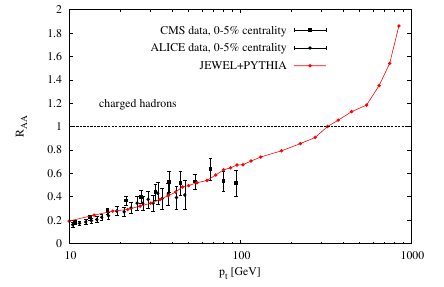
\includegraphics[width=0.8\textwidth]{images/charged_hadron_supression.png}
\caption[Charged Hadron $R_{AA}$]{Hadron $R_{AA}$ as measured by CMS and ALICE collaborations compared to JEWEL predictions. Figure from \cite{zapp_perturbative_2013}.}
\label{charged_hadron_supression}
\end{figure}

\begin{figure}
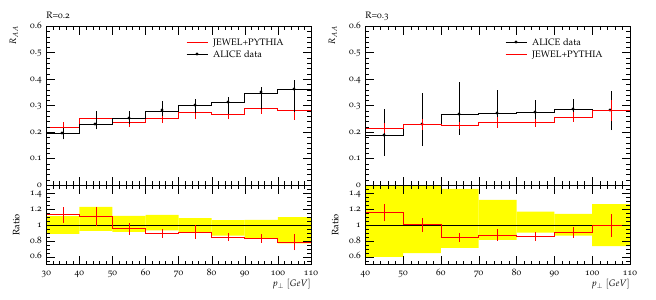
\includegraphics[width=1.0\textwidth]{images/jewel_jetpt_supression.png}
\caption[JEWEL prediction of $R_{AA}$ for the jet $p_t$.]{Jet $p_T$ $R_{AA}$ as measured by CMS, ALICE and ATLAS collaborations compared to JEWEL predictions. Figure from \cite{zapp_perturbative_2013}.}
\label{jewel_jetpt_supression}
\end{figure}

Studying internal jet structure, we can see a somewhat different picture of JEWEL performance. For instance, in Figure \ref{jewel_girth} we see that JEWEL predicts jets broader than data. In the case of jet mass, we see on Figure \ref{jewel_mass}. We are interested in this work in the case with the recoiling scattering centers, since radiation patterns trying to probe the medium is our goal. JEWEL also predicts higher values for this observable, indicating broader jets than expected. In the case without recoils, the jet mass has lower values than data, which indicates a hardening of the core.

\begin{figure}
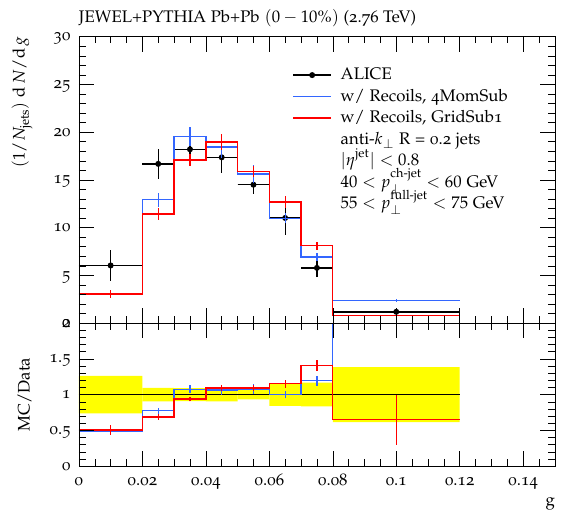
\includegraphics[width=1.0\textwidth]{images/jewel_girth.png}
\caption[JEWEL prediction for girth.]{JEWEL predictions for jet girth compared to measurements from ALICE collaboration. Figure from \cite{elayavalli_medium_2017}.}
\label{jewel_girth}
\end{figure}

\begin{figure}
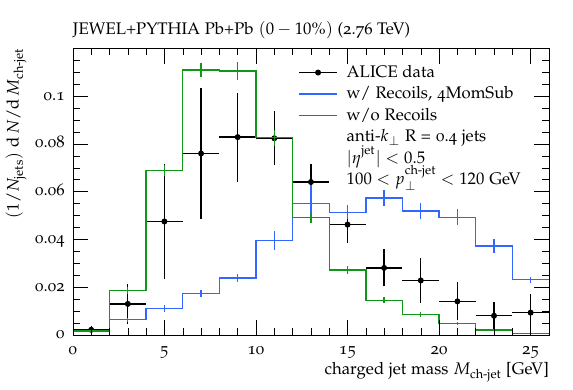
\includegraphics[width=1.0\textwidth]{images/jewel_mass.png}
\caption[JEWEL prediction for mass.]{JEWEL predictions for jet mass compared to measurements from ALICE collaboration. Figure from \cite{elayavalli_medium_2017}.}
\label{jewel_mass}
\end{figure}

\mysection{JEWEL with realistic IC} \label{jewel_with_ic}

In Figure \ref{jet_girth_ic} we see the results for jet girth with realistic initial conditions. Here $\rm T_RENTo$ was used with calibration to fit IP-Glasma results\cite{moreland_alternative_2015}. JEWEL tends to overestimate the peak value even with the new initial conditions. One is reminded that girth is related to the angular opening of the jet. Girth also depends linearly on the transverse momenta of the particles. The overestimation of JEWEL results tells us that the jets produced by the simulation tend to be slightly broader than the jets from data. No further improvement comes from the inclusion of more realistic initial conditions, as the results given by the inclusion of realistic initial conditions agree with the default of JEWEL.

\begin{figure}
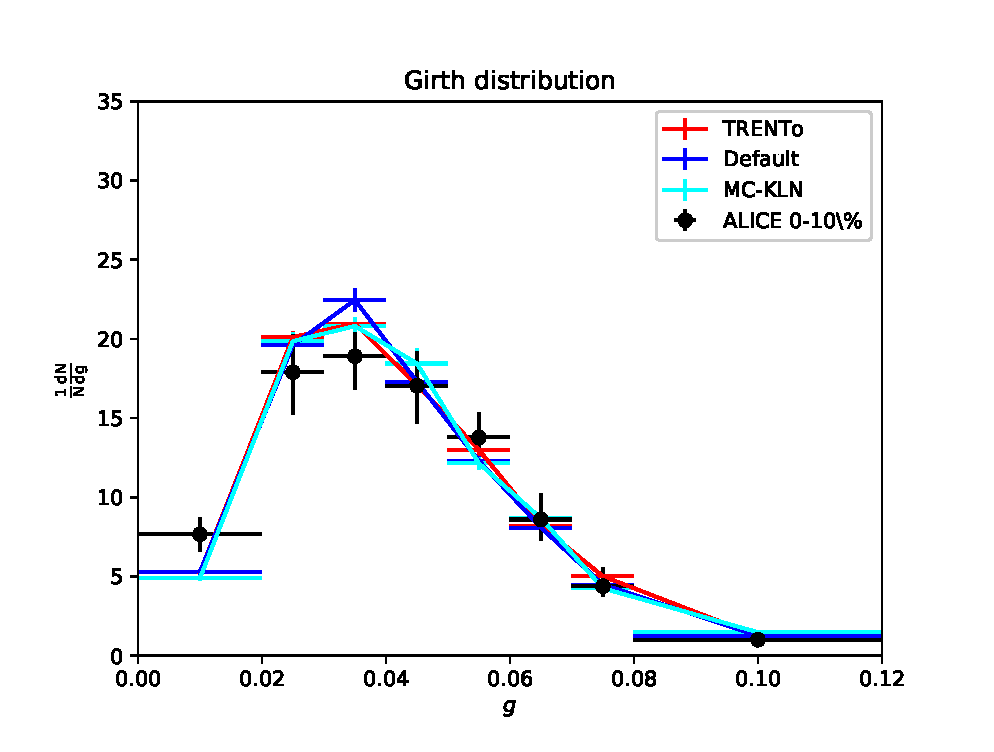
\includegraphics[width=1.0\textwidth]{images/My_Angularity_3.eps}
\caption[Jet Girth with realistic IC]{Jet Girth for charged jets calculated for $R=0.2$ anti-kt algorithm and $|\eta|<0.8$. $40 {\rm GeV/c} < p_T < 60 {\rm GeV}$. The CM energy is $\sqrt{s_{NN}}= 2.76 {\rm TeV}$. On the $0-10\%$ centrality class.}
\label{jet_girth_ic}
\end{figure}

In Figure \ref{jet_dispersion_ic} we see the results for the jet dispersion. The default of JEWEl predicts slightly lower values than data. This indicates softer fragmentation. With the inclusion of realistic initial conditions, there is no substantial difference.

\begin{figure}
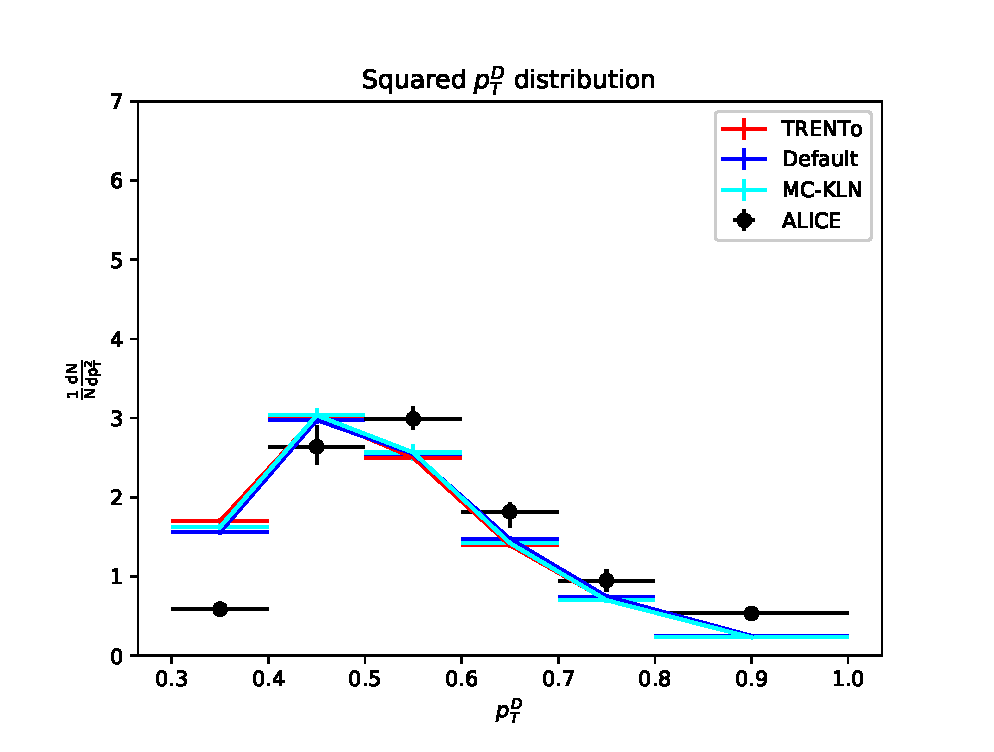
\includegraphics[width=1.0\textwidth]{images/Squared_3.eps}
\caption[Jet $p_D^T$ with realistic IC]{Jet Dispersion for charged jets calculated for $R=0.2$ anti-kt algorithm and $|\eta|<0.8$. $40 {\rm GeV/c} < p_T < 60 {\rm GeV}$. The CM energy is $\sqrt{s_{NN}}= 2.76 {\rm TeV}$. On the $0-10\%$ centrality class.}
\label{jet_dispersion_ic}
\end{figure}

The results for the jet mass are displayed in Figure \ref{jet_mass_ic}. Here we present also the inclusion of realistic IC for this observable. JEWEL in its default does not make a good prediction for it already. The problem is of the same nature of the disagreement of the girth, but worst. The jets in data tend to have a lower mass than predicted, this indicates larger jets, as is the case with girth. The mass further indicates that the problem lies in the soft fragmentation, which depends strongly on hadronization. There is some improvement from the addition of the realistic IC background, as one can see from the slight shift to the left. This shift is not significant though, due to the uncertainties of the method. There is a discrepancy in the spectrum. 

\begin{figure}
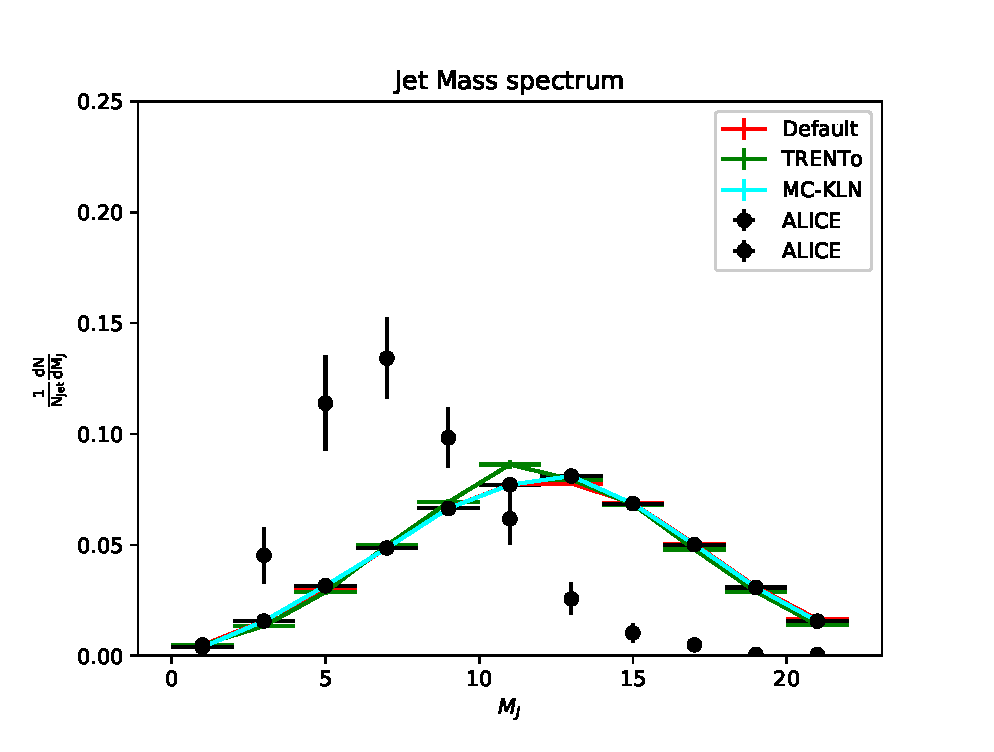
\includegraphics[width=1.0\textwidth]{images/Mass_3.eps}
\caption[Jet Mass with realistic IC]{Jet Mass for charged jets calculated for $R=0.2$ anti-kt algorithm and $|\eta|<0.8$. $40 {\rm GeV/c} < p_T < 60 {\rm GeV}$. The CM energy is $\sqrt{s_{NN}}= 2.76 {\rm TeV}$. On the $0-10\%$ centrality class.}
\label{jet_mass_ic}
\end{figure}

In Figure \ref{jet_v2_ic} we see the results for the jet $v_2$. The data from ALICE and ATLAS show that there is tension between the experimental results making any conclusion about the performance of the model more difficult. ALICE uses their TPCs for jet reconstruction and ATLAS uses the hadronic calorimeters. This means that ALICE uses only charged particles, and ATLAS uses all hadrons for jet reconstruction. This explains why ALICE data has lower values of $p_T$. Although there is a disagreement between the collaborations, both data seems to indicate that the $v_2$ is different from zero. This is expected from fluctuations that happen on the initial conditions, since central collisions don't have a geometry that naturally raises an azimuthal asymmetry on the energy distribution. We can see in the Figure \ref{jet_v2_ic} that JEWEL, even with realistic IC, predicts values consistent with zero $v_2$.

\begin{figure}
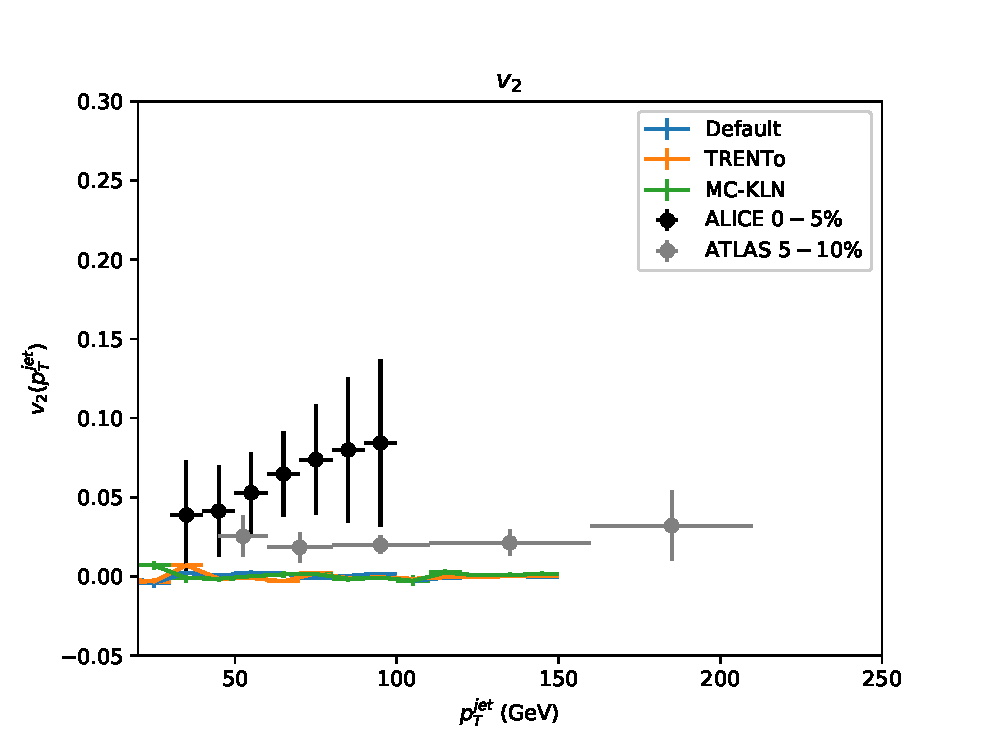
\includegraphics[width=1.0\textwidth]{images/v2_4.eps}
\caption[Jet $v_2$ with realistic IC]{Jet $v_2$ calculated for $R=0.4$ anti-kt algorithm and $|\eta|<0.8$. The CM energy is $\sqrt{s_{NN}}= 2.76 {\rm TeV}$. On the $0-10\%$ centrality class.}
\label{jet_v2_ic}
\end{figure}

\mysection{JEWEL with realistic hydro} \label{jewel_with_hydro}

In Figure \ref{jet_girth} we see the results for jet girth. Considering the hydrodynamic expansion for the medium as well. The result shows that JEWEL tends to overestimate it. Since girth is related to the jet width, this shows broader jets than the data. No further improvement comes from the inclusion of more realistic initial conditions or hydrodynamics, as the results given by the inclusion of the realistic hydro and initial conditions agree with the default of JEWEL.

\begin{figure}
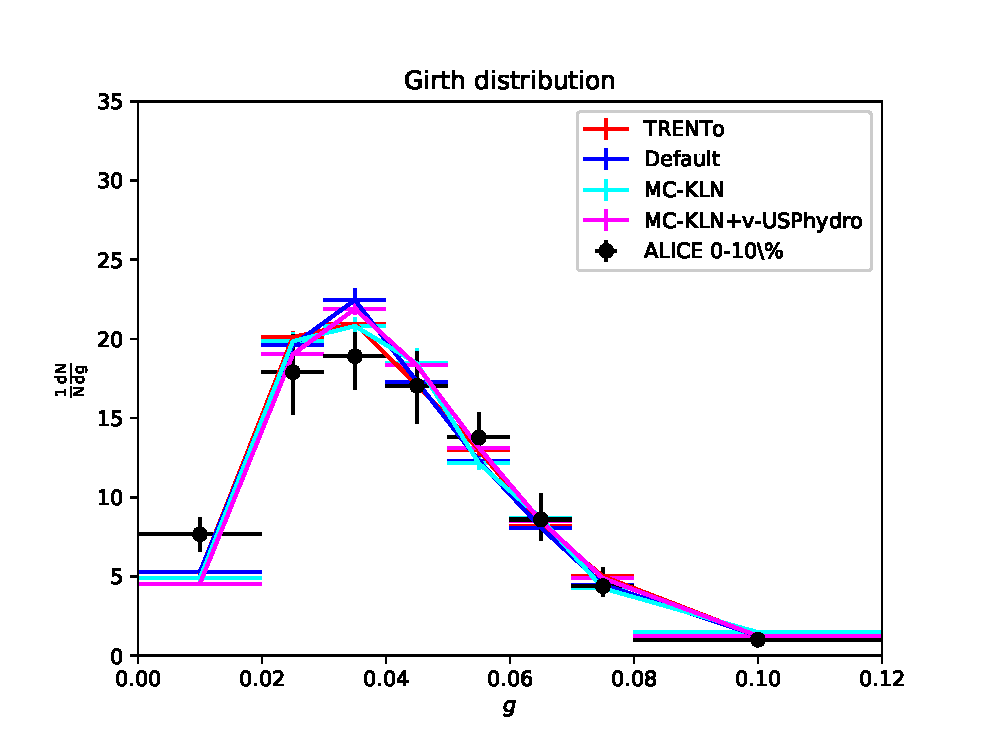
\includegraphics[width=1.0\textwidth]{images/My_Angularity_4.eps}
\caption[Jet Girth]{Jet Girth for charged jets calculated for $R=0.2$ anti-kt algorithm and $|\eta|<0.8$. $40 {\rm GeV/c} < p_T < 60 {\rm GeV}$. The CM energy is $\sqrt{s_{NN}}= 2.76 {\rm TeV}$. On the $0-10\%$ centrality class.}
\label{jet_girth}
\end{figure}

In Figure \ref{jet_dispersion} we see the results for the jet dispersion with the inclusion of realistic hydro. The default of JEWEl predicts slightly lower values than data. This indicates softer fragmentation. With the inclusion of realistic hydro, the agreement is slightly worst for lower values, but not substantially different. This indicates that the fragmentation is slightly softer than that of the default. Regions of greater density on the profile could be responsible for the further soft radiation causing this.

\begin{figure}
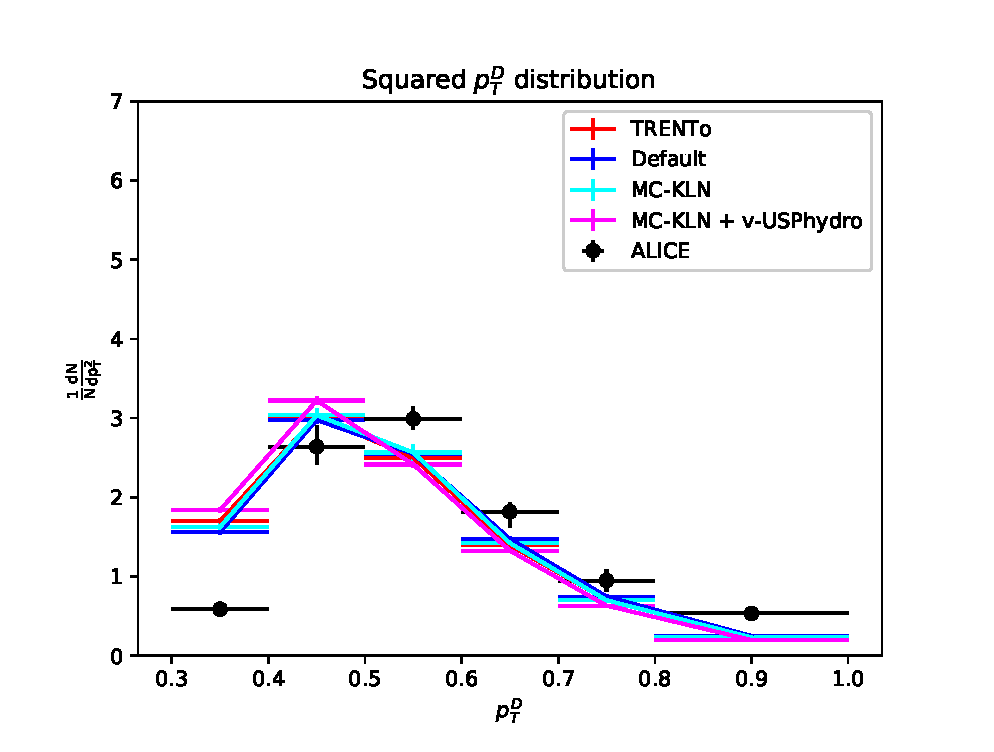
\includegraphics[width=1.0\textwidth]{images/Squared_4.eps}
\caption[Jet $p_D^T$]{Jet Dispersion for charged jets calculated for $R=0.2$ anti-kt algorithm and $|\eta|<0.8$. $40 {\rm GeV/c} < p_T < 60 {\rm GeV}$. The CM energy is $\sqrt{s_{NN}}= 2.76 {\rm TeV}$. On the $0-10\%$ centrality class.}
\label{jet_dispersion}
\end{figure}

The results for the jet mass are displayed in Figure \ref{jet_mass}. JEWEL in its default doesn't make a good prediction for it. The problem is of the same nature of the disagreement of the girth, but worst. The jets in data tend to have a lower mass than predicted, this indicates larger jets, as is the case with girth. The mass further indicates that the problem lies in the soft fragmentation, which depends strongly on hadronization. There is some improvement from the addition of the realistic hydrodynamics background, although there is a discrepancy in the spectrum. 

\begin{figure}
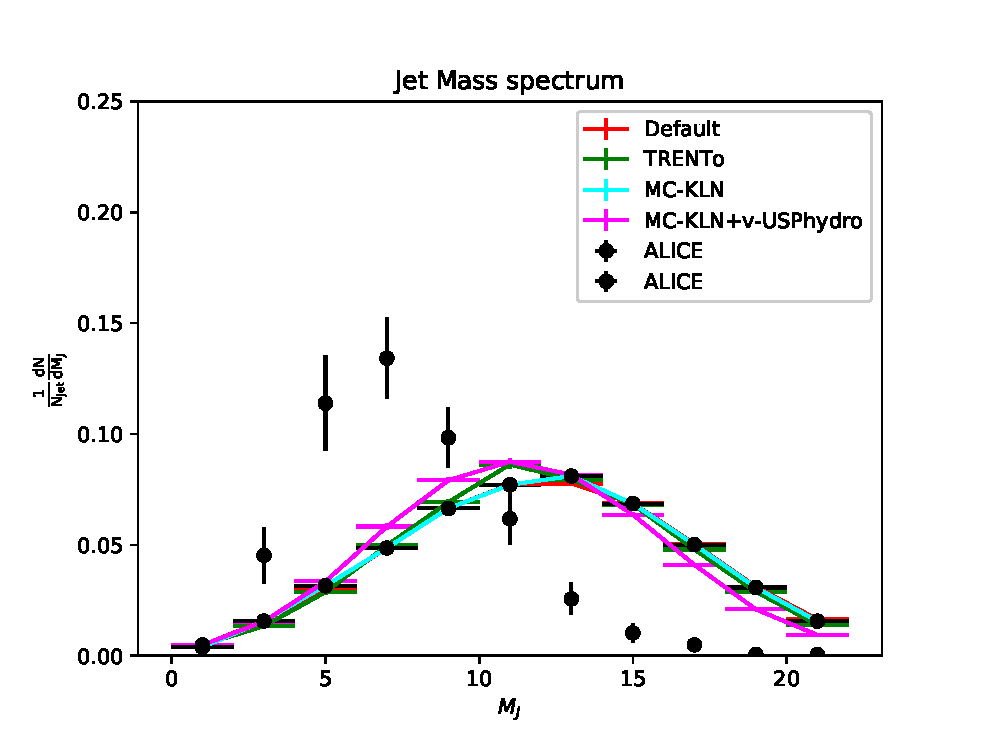
\includegraphics[width=1.0\textwidth]{images/Mass_4.eps}
\caption[Jet Mass]{Jet Mass for charged jets calculated for $R=0.2$ anti-kt algorithm and $|\eta|<0.8$. $40 {\rm GeV/c} < p_T < 60 {\rm GeV}$. The CM energy is $\sqrt{s_{NN}}= 2.76 {\rm TeV}$. On the $0-10\%$ centrality class.}
\label{jet_mass}
\end{figure}

In Figure \ref{jet_v2} we see the results for the jet $v_2$, with the inclusion of realistic hydro. Although there is a disagreement between the collaborations, both data seems to indicate that the $v_2$ is different from zero. The fluctuations might be responsible for the existence of the asymmetry. We can see in Figure \ref{jet_v2} that the inclusion of the realistic hydro has raised the $v_2$ from zero, although there seems to be overestimating it. The simulations currently performed tell us that the combined effect of realistic initial conditions and hydrodynamics are responsible for this effect. The fact that neither MC-KLN nor $\rm T_RENTo$ have shown significant $v_2$ indicates that the hydrodynamics is an essential ingredient for describing this observable.

\begin{figure}
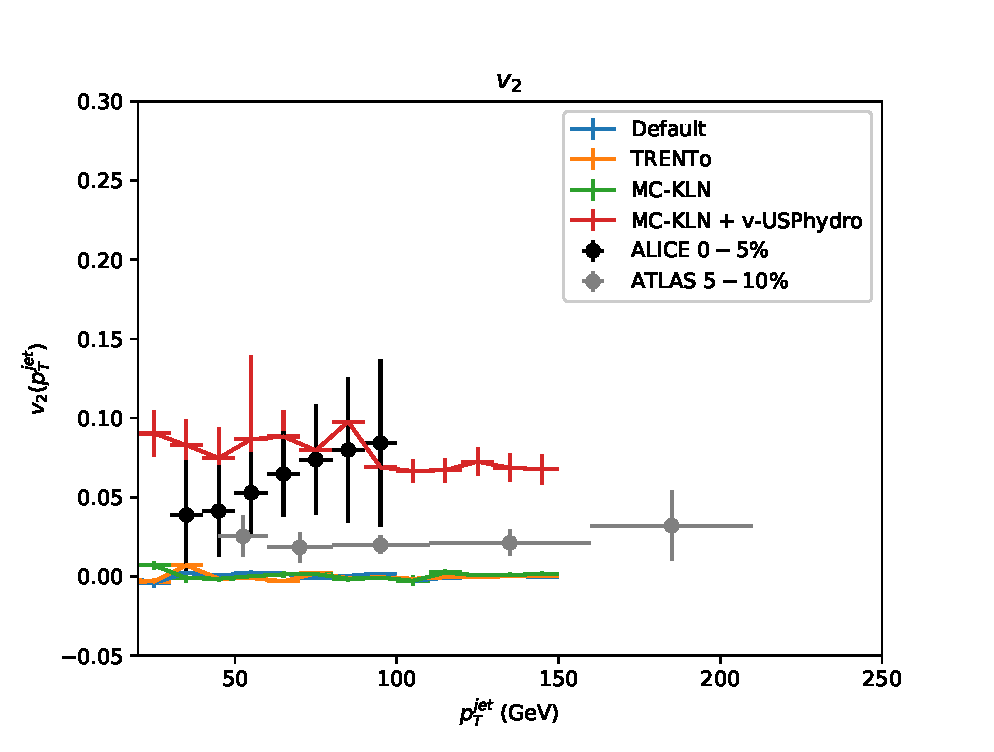
\includegraphics[width=1.0\textwidth]{images/v2_5.eps}
\caption[Jet $v_2$]{Jet $v_2$ calculated for $R=0.4$ anti-kt algorithm and $|\eta|<0.8$. The CM energy is $\sqrt{s_{NN}}= 2.76 {\rm TeV}$. On the $0-10\%$ centrality class.}
\label{jet_v2}
\end{figure}